% ---
% Packages
% ---
\documentclass[11pt,a4paper,twoside,onecolumn]{book}
\usepackage[utf8]{inputenc}
\usepackage[strict]{changepage}
\usepackage{xcolor}
\usepackage{framed}
\usepackage{fourier}
\usepackage{graphicx}
\usepackage{geometry}
\usepackage{layout}
\usepackage{pifont}
\usepackage{fontawesome}
\usepackage{float}
\usepackage{longtable}

\definecolor{formalshade}{rgb}{0.95,0.95,1}

\newenvironment{formalred}{%
	\def\FrameCommand{%
		\hspace{1pt}%
		{\color{red}\vrule width 2pt}%
		{\color{formalshade}\vrule width 4pt}%
		\colorbox{formalshade}%
	}%
	\MakeFramed{\advance\hsize-\width\FrameRestore}%
	\noindent\hspace{-4.55pt}% disable indenting first paragraph
	\begin{adjustwidth}{}{7pt}%
		\vspace{2pt}\vspace{2pt}%
	}
	{%
		\vspace{2pt}\end{adjustwidth}\endMakeFramed%
}

\newenvironment{formalblue}{%
	\def\FrameCommand{%
		\hspace{1pt}%
		{\color{blue}\vrule width 2pt}%
		{\color{formalshade}\vrule width 4pt}%
		\colorbox{formalshade}%
	}%
	\MakeFramed{\advance\hsize-\width\FrameRestore}%
	\noindent\hspace{-4.55pt}% disable indenting first paragraph
	\begin{adjustwidth}{}{7pt}%
		\vspace{2pt}\vspace{2pt}%
	}
	{%
		\vspace{2pt}\end{adjustwidth}\endMakeFramed%
}

\newenvironment{formalyellow}{%
	\def\FrameCommand{%
		\hspace{1pt}%
		{\color{yellow}\vrule width 2pt}%
		{\color{formalshade}\vrule width 4pt}%
		\colorbox{formalshade}%
	}%
	\MakeFramed{\advance\hsize-\width\FrameRestore}%
	\noindent\hspace{-4.55pt}% disable indenting first paragraph
	\begin{adjustwidth}{}{7pt}%
		\vspace{2pt}\vspace{2pt}%
	}
	{%
		\vspace{2pt}\end{adjustwidth}\endMakeFramed%
}

\geometry{
	top=20mm,
	bottom=25mm,
	left=20mm,
	right=20mm,
	bindingoffset=15mm,	
}

% ---
% PDF Information
% ---
\title{Manual Pengguna - Elbicare Audiometers}

% ---
% Document Content
% ---

\begin{document}
	
	\maketitle
	
	\begin{figure}[H]
		\centering
		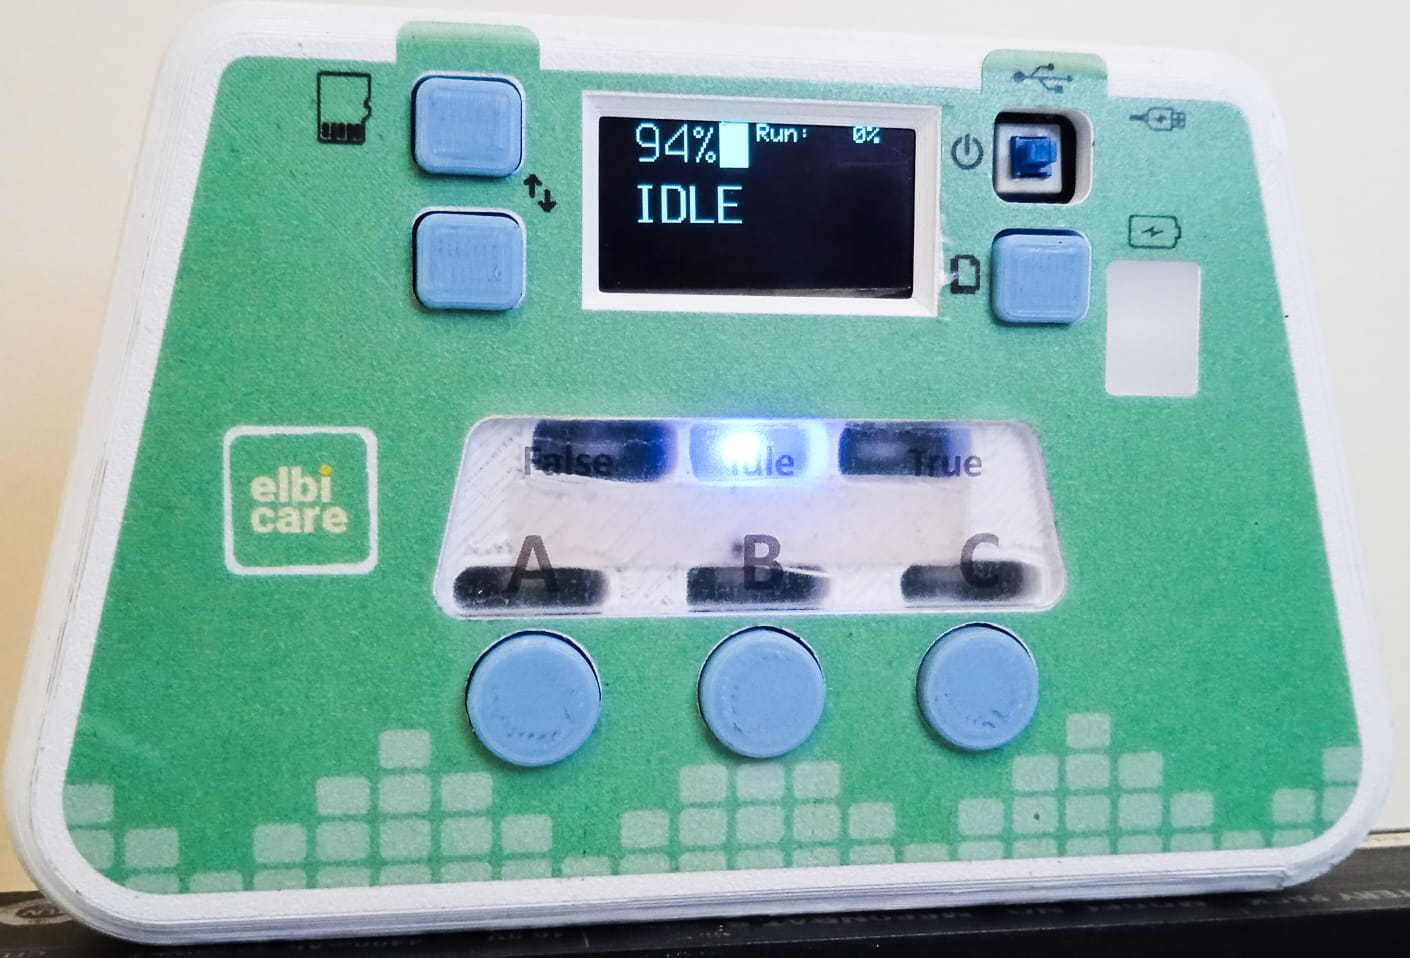
\includegraphics[width=\columnwidth]{images/depan-idle}
	\end{figure}

	\begin{figure}[H]
		\centering
		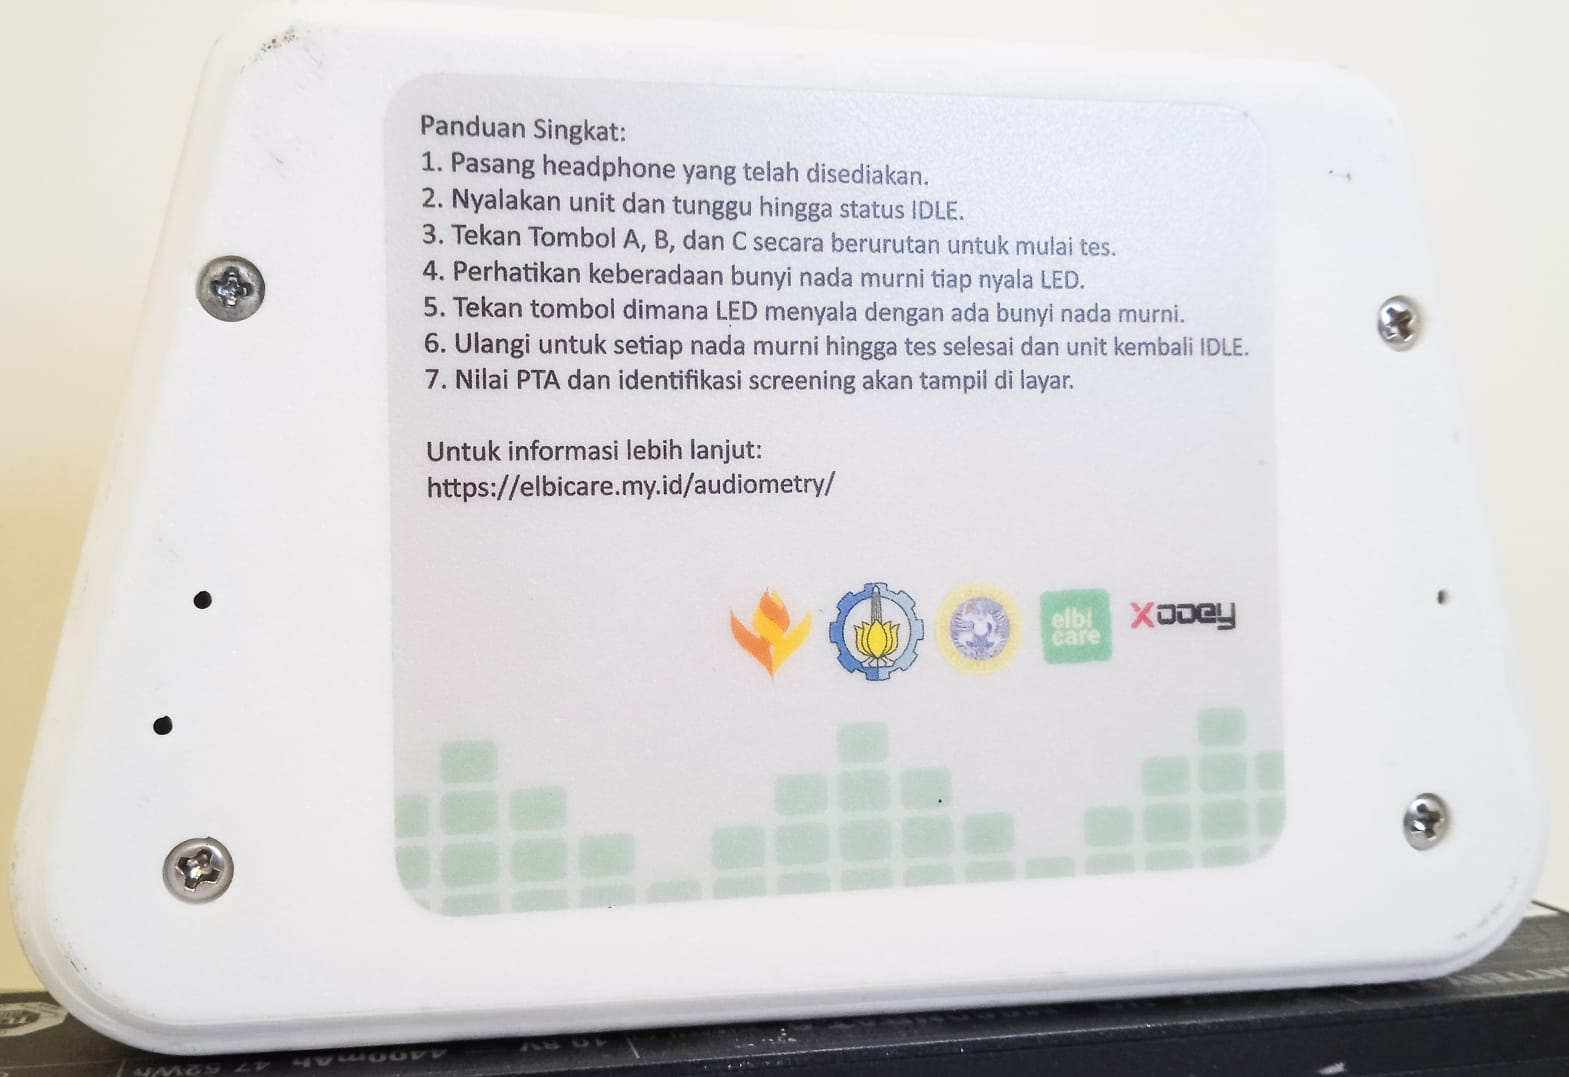
\includegraphics[width=\columnwidth]{images/belakang}
	\end{figure}
	
	\renewcommand\contentsname{Daftar Isi}
	\tableofcontents
	\addcontentsline{toc}{chapter}{Daftar Isi}
	
	\renewcommand\listfigurename{Daftar Gambar}
	\listoffigures
	\addcontentsline{toc}{chapter}{Daftar Gambar}
	
	\renewcommand\listtablename{Daftar Tabel}
	\listoftables
	\addcontentsline{toc}{chapter}{Daftar Tabel}
	\newpage
	
	\renewcommand\chaptername{Bab}
	
	\chapter{Pendahuluan}
		\section{Tujuan Manual}
		Dokumen ini berisi informasi penting mengenai petunjuk pengoperasian perangkat Elbicare Audiometer secara aman. Perangkat ini merupakan perangkat elektronik yang dapat bekerja selama beberapa tahun dengan pengoperasian yang cermat, sesuai dengan deskripsi pada dokumen ini. Pastikan untuk membaca dan memahami instruksi pada manual ini sebelum mengoperasikan perangkat Elbicare Audiometer. 
		
		\begin{formalred}
			\raisebox{0.325ex}{\resizebox{!}{2ex}{\danger}} \textbf{PERINGATAN}:
			Sebelum memulai mengoperasikan perangkat ini, silahkan baca, pahami, dan ikuti dengan seksama informasi pada Bab~\ref{chap:2} Informasi Keselamatan 
		\end{formalred}
		
		\section{Jenis Alat}
		\begin{tabular}{lcl}
			Merek & : & Elbicare Audiometer\\
			Model & : & v3.0\\
			No. Seri & : & \\
		\end{tabular}
		
		\section{Informasi Produsen}
		\begin{tabular}{l}
			\textbf{\textcolor{blue}{PT. Xirka Dama Persada}}\\
			Gedung CM, Jl. Mataram I No. 9 Jakarta Timur, 13150, Indonesia\\
			Telepon +62-21-819-8700; Fax. +62-21-2850-7071\\
			Email: info@xooey.id\\
		\end{tabular}
		
		\section{Pelayanan Purna Jual}
		Elbicare Audiometer menawarkan servis purna jual atau garansi sejak perangkat dibeli. Detail mengenai informasi ini dapat diperoleh dengan menghubungi \textcolor{blue}{PT. Xirka Dama Persada}.
		
		
	\newpage
	
	\chapter{Informasi Keselamatan}\label{chap:2}
		\section{Definisi}
		Dokumen Manual ini menggunakan tiga jenis indikator untuk memperjelas informasi penting berupa: peringatan, perhatian, dan juga catatan. Ketiga hal tersebut muncul dengan bentuk sebagaimana ditunjukkan pada Tabel ~\ref{tab:2.1}
		
		\begin{table}[H]
			\centering
			\caption{Indikator dalam Buku Manual Pengguna}
			\label{tab:2.1}
			\begin{tabular}{|p{0.15\linewidth}  | p{0.7\linewidth}|}
				\hline
				Simbol & Keterangan\\
				\hline
				\hline
				\resizebox{!}{4ex}{\danger} & PERINGATAN: \linebreak 
				Mengindikasikan kondisi yang dapat membahayakan pasien atau operator perangkat\\
				\hline
				\resizebox{!}{4ex}{\faSearch} & PERHATIAN: \linebreak
				Mengindikasikan kondisi yang dapat merusak atau mengurangi masa pakai perangkat \\
				\hline
				\resizebox{!}{4ex}{\ding{46}} & CATATAN: \linebreak
				Mengindikasikan informasi yang dapat menjadikan pengoperasian menjadi lebih efisien dan optimal\\
				\hline
			\end{tabular}
		\end{table}
	
		Untuk dapat mengoperasikan perangkat secara tepat dan efisien, dan untuk mencegah insiden, dimohon untuk memberikan perhatian khusus pada bagian ~\ref{sec:2.2} Peringatan, serta semua peringatan dan perhatian yang ada di manual ini.
		
		\begin{formalblue}
			\raisebox{0.1ex}{\resizebox{!}{2.5ex}{\ding{46}}} \textbf{CATATAN}:
			Untuk bantuan lebih lanjut, hubungi perwakilan dari \textcolor{blue}{PT. Xirka Dama Persada} 
		\end{formalblue}
		
		\section{Peringatan}\label{sec:2.2}
			\subsection{Peringatan Umum Mengenai Penggunaan Alat}
				\begin{formalred}
					\raisebox{0.125ex}{\resizebox{!}{2ex}{\danger}} \textbf{PERINGATAN}:
					Perangkat hanya dapat digunakan di bawah tanggung jawab dan rekomendasi dokter dan hanya boleh digunakan untuk kegunaan semestinya seperti tertulis pada Bab 3.1 Indikasi Penggunaan. 
				\end{formalred}
			
				\begin{formalred}
					\raisebox{0.125ex}{\resizebox{!}{2ex}{\danger}} \textbf{PERINGATAN}: 
					Manual ini menjelaskan cara merespon terhadap perangkat, tidak menjelaskan cara penanganan pasien. 
				\end{formalred}
			
				\begin{formalred}
					\raisebox{0.125ex}{\resizebox{!}{2ex}{\danger}} \textbf{PERINGATAN}: 
					Untuk menjamin kinerja perangkat secara optimal, pastikan baterai telah melalui proses charging.
				\end{formalred}
				
				\begin{formalred}
					\raisebox{0.125ex}{\resizebox{!}{2ex}{\danger}} \textbf{PERINGATAN}: 
					Gunakan hasil koreksi yang ditampilkan pada sertifikat kalibrasi yang dikeluarkan oleh institusi yang berwenang
				\end{formalred}
			
				\begin{formalred}
					\raisebox{0.125ex}{\resizebox{!}{2ex}{\danger}} \textbf{PERINGATAN}: 
					Jangan mulai menyalakan perangkat kecuali perangkat telah dirakit dengan benar, tidak tampak cacat fisik pada perangkat
				\end{formalred}
			
				\begin{formalred}
					\raisebox{0.125ex}{\resizebox{!}{2ex}{\danger}} \textbf{PERINGATAN}: 
					Gunakan perangkat tambahan hanya yang direkomendasikan oleh manual ini. Ada kemungkinan ketidakcocokan atau bahkan tidak aman jika menghubungkan perangkat dengan perangkat lain yang tidak direkomendasikan oleh manual ini.
				\end{formalred}
			
				\begin{formalred}
					\raisebox{0.125ex}{\resizebox{!}{2ex}{\danger}} \textbf{PERINGATAN}: 
					Untuk mengurangi risiko infeksi, cuci tangan dengan baik sebelum maupun setelah memegang perangkat atau aksesorinya.
				\end{formalred}
			
				\begin{formalred}
					\raisebox{0.125ex}{\resizebox{!}{2ex}{\danger}} \textbf{PERINGATAN}: 
					Perangkat dan aksesori yang kotor dapat menjadi sumber infeksi. Bersihkan perangkat dan aksesorinya sebelum dan setelah penggunaan, secara regular dan sistematis, serta mengikuti prosedur perawatan untuk mengurangi risiko infeksi. Cek di Bab 7, Petunjuk Pembersihan.
				\end{formalred}
			
				\begin{formalred}
					\raisebox{0.125ex}{\resizebox{!}{2ex}{\danger}} \textbf{PERINGATAN}: 
					Gunakan perangkat dengan hati-hati selama dan setelah penggunaan, terutama jika temperatur lingkungan relatif tinggi. Sebagian permukaan perangkat temperaturnya dapat sedikit meningkat, walaupun penggunaan masih dalam batas aman.
				\end{formalred}
			
				\begin{formalred}
					\raisebox{0.125ex}{\resizebox{!}{2ex}{\danger}} \textbf{PERINGATAN}: 
					Tidak dibolehkan memodifikasi peralatan ini.
				\end{formalred}
			
				\begin{formalred}
					\raisebox{0.125ex}{\resizebox{!}{2ex}{\danger}} \textbf{PERINGATAN}: 
					Peralatan ini tidak boleh dimodifikasi tanpa seizin pabrik. Apabila mendapatkan modifikasi tanpa persetujuan pabrik, tidak ada jaminan bahwa mesin dapat berfungsi dengan semestinya.
				\end{formalred}
			
				\begin{formalred}
					\raisebox{0.125ex}{\resizebox{!}{2ex}{\danger}} \textbf{PERINGATAN}: 
					Jika peralatan ini dimodifikasi, inspeksi dan pengujian yang sesuai harus dilakukan untuk memastikan peralatan aman untuk digunakan.
				\end{formalred}
			
				\begin{formalred}
					\raisebox{0.125ex}{\resizebox{!}{2ex}{\danger}} \textbf{PERINGATAN}: 
					Perangkat tidak boleh direndam di cairan apa pun. Cairan yang terdapat di permukaan perangkat harus dilap sesegera mungkin. Untuk menghindari kerusakan, cairan tidak boleh masuk ke perangkat.
				\end{formalred}
			
				\begin{formalred}
					\raisebox{0.125ex}{\resizebox{!}{2ex}{\danger}} \textbf{PERINGATAN}: 
					Untuk memastikan pengoperasian yang benar sehingga perangkat menjadi awet, pastikan perangkat beroperasi pada kondisi lingkungan yang direkomendasikan.
				\end{formalred}
			
				\begin{formalred}
					\raisebox{0.125ex}{\resizebox{!}{2ex}{\danger}} \textbf{PERINGATAN}: 
					Jangan operasikan perangkat di lingkungan magnetic resonance imaging (MRI), di bawah sinar matahari langsung, di dekat sumber panas, di dekat perangkat bedah yang memiliki High Frequency(HF) aktif, di luar ruangan, di dekat instalasi cairan tanpa proteksi, maupun di area berdebu.
				\end{formalred}
			
				\begin{formalred}
					\raisebox{0.125ex}{\resizebox{!}{2ex}{\danger}} \textbf{PERINGATAN}: 
					Pastikan sekeliling perangkat memungkinkan instalasi dan operasi perangkat secara baik
				\end{formalred}
			
				\begin{formalred}
					\raisebox{0.125ex}{\resizebox{!}{2ex}{\danger}} \textbf{PERINGATAN}: 
					Pastikan pemasangan perangkat ada di lokasi yang sulit dijangkau oleh anak-anak, hewan peliharaan, maupun hewan liar, dan sesuatu yang dapat menimbulkan bahaya dan kerusakan pada perangkat
				\end{formalred}
			
				\begin{formalred}
					\raisebox{0.125ex}{\resizebox{!}{2ex}{\danger}} \textbf{PERINGATAN}: 
					Untuk mengurangi risiko terbakar, jauhkan perangkat dari rokok yang menyala, korek api, dan sumber pembakaran lainnya.
				\end{formalred}			
				
			\subsection{Peringatan Mengenai Sistem Kelistrikan}
				\begin{formalred}
					\raisebox{0.125ex}{\resizebox{!}{2ex}{\danger}} \textbf{PERINGATAN}: 
					Pengisian ulang daya baterai secara rutin penting untuk memaksimalkan usia baterai. Jika tersimpan terlalu lama tanpa diisi ulang dayanya, usia baterai dapat berkurang.
				\end{formalred}
				
				\begin{formalred}
					\raisebox{0.125ex}{\resizebox{!}{2ex}{\danger}} \textbf{PERINGATAN}: 
					Catu daya listrik harus sesuai dengan spesifikasi perangkat. Pastikan tidak ada kabel yang terlipat maupun tertekan. Perangkat sebaiknya tidak dinyalakan ketika kabel listrik AC rusak. 
				\end{formalred}
				
				\begin{formalred}
					\raisebox{0.125ex}{\resizebox{!}{2ex}{\danger}} \textbf{PERINGATAN}: 
					Jangan mendekatkan perangkat pada api. Pembuangan limbah baterai harus sesuai dengan peraturan lokal yang berlaku.
				\end{formalred}
			
			\subsection{Peringatan Mengenai Peraturan}
				\begin{formalred}
					\raisebox{0.125ex}{\resizebox{!}{2ex}{\danger}} \textbf{PERINGATAN}: 
					Sebelum mulai proses audiometri, pastikan semua pengaturan sesuai dengan buku manual pengguna ini. Pastikan juga instalasi dilakukan dengan benar.
				\end{formalred}
				
				\begin{formalred}
					\raisebox{0.125ex}{\resizebox{!}{2ex}{\danger}} \textbf{PERINGATAN}: 
					Gunakan hasil koreksi yang ditampilkan pada sertifikat kalibrasi yang dikeluarkan oleh institusi yang berwenang
				\end{formalred}	
			
		\section{Simbol, Label, dan Penanda}
		Simbol, label, dan penanda pada perangkat Elbicare Audiomters ditunjukkan melalui tabel berikut.
		
			\begin{longtable}{| p{0.3\linewidth} | p{0.2\linewidth}| p{0.4\linewidth}|}
				\hline
				\textbf{Simbol} & \textbf{Lokasi} & \textbf{Deskripsi} \\
				\hline
				\endfirsthead
				\hline
				\textbf{Simbol} & \textbf{Lokasi} & \textbf{Deskripsi} \\
				\hline
				\endhead
				\hline
				\multicolumn{3}{r}{\textit{Continued on next page}} \\
				\endfoot
				\hline
				\endlastfoot

				\hline
				
\includegraphics[width=0.1\textwidth]{images/powerswitch} & Panel Depan & Tombol \emph{power switch} untuk menyakalakan perangkat audiometer\\
				\hline
				
\includegraphics[width=0.1\textwidth]{images/user-mode} & Panel Depan & Tombol \emph{user mode}\\
				\hline
				
\includegraphics[width=0.1\textwidth]{images/user-action} & Panel Depan & Tombol \emph{user action}\\
				\hline
				
\includegraphics[width=0.1\textwidth]{images/penanda-merk} & Panel Depan & Penanda merk\\
				\hline
				
\includegraphics[width=0.1\textwidth]{images/3-forced-choice} & Panel Depan & Tombol 3-\emph{Force choice}\\
				\hline
				
\includegraphics[width=0.1\textwidth]{images/true} & Panel Depan & Lampu indikator jawaban benar\\
				\hline
				
\includegraphics[width=0.1\textwidth]{images/false} & Panel Depan & Lampu indikator jawaban salah\\
				\hline
				
\includegraphics[width=0.1\textwidth]{images/idle} & Panel Depan & Lampu indikator kondisi idle\\
				\hline
				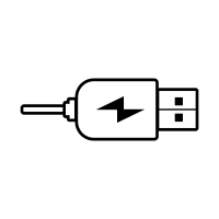
\includegraphics[width=0.1\textwidth]{images/charging-port} & Panel Depan & \emph{Port} pengisian daya baterai (\emph{battery charger})\\
				\hline
				
\includegraphics[width=0.1\textwidth]{images/charging-indicator} & Panel Depan & Lampu indikator pengisian daya baterai (\emph{battery charger})\\
				\hline
				
\includegraphics[width=0.1\textwidth]{images/usb-data-interface} & Panel Depan & \emph{Port} USB \emph{data interface}\\
				\hline
				
\includegraphics[width=0.1\textwidth]{images/micro-SD} & Panel Depan & \emph{Port} micro-SD \emph{slot}\\
				\hline
				
\includegraphics[width=0.1\textwidth]{images/lpdp} & Panel Belakang & Logo pemberi dana hibah\\
				\hline
				
\includegraphics[width=0.1\textwidth]{images/its} & Panel Belakang & Logo insitusi pengembang (\emph{research and development})\\
				\hline
				
\includegraphics[width=0.1\textwidth]{images/unair} & Panel Belakang & Logo insitusi pengembang (\emph{research and development})\\
				\hline
				
\includegraphics[width=0.1\textwidth]{images/penanda-merk} & Panel Belakang & Penanda merk\\
				\hline
				
\includegraphics[width=0.2\textwidth]{images/xirka} & Panel Belakang & Logo penyedia jasa produksi dan pelayanan purna jual\\
				\hline
				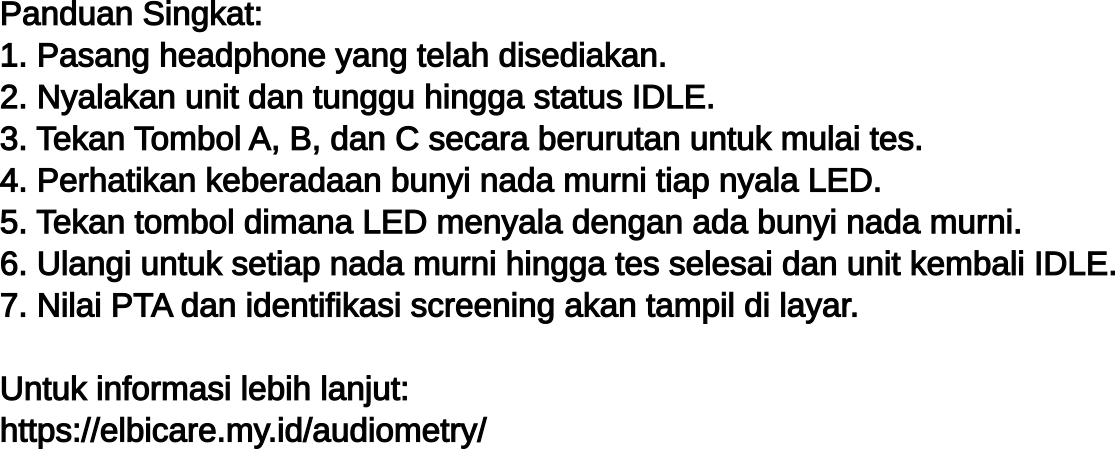
\includegraphics[width=0.3\textwidth]{images/manual} & Panel Belakang & Informasi panduan singkat\\
				\hline
			\end{longtable}
		
	\newpage
	
	\chapter{Overview Sistem}
		\section{Indikasi Penggunaan}
		Elbicare Audiometer dimaksudkan untuk digunakan sebagai alat screening kondisi pendengaran manusia. Perangkat ini ditujukan untuk digunakan langsung oleh pasien dengan izin dokter. Berkaitan dengan penggunaan secara langsung, pasien selaku pengguna perlu membaca, memahami, dan mengikuti instruksi di manual ini sebelum menggunakan perangkat Elbicare Audiometer.
			\subsection{Target Pasien}
			Elbicare Audiometer ini ditujukan kepada orang/pasien yang dianggap memerlukan screening kondisi pendengaran oleh dokter atau institusi tertentu.
			\subsection{Target Lingkungan Pengoperasian}
			Elbicare Audiometer ini ditujukan untuk digunakan di lokasi statis seperti di rumah sakit, ruangan medis, dan rumah pasien. Perangkat ini dapat bekerja di lingkungan dengan bising latar belakang maksimal senilai \textbf{58 dB}. 
			
			\begin{formalred}
				\raisebox{0.125ex}{\resizebox{!}{2ex}{\danger}} \textbf{PERINGATAN}: 
				Jangan gunakan Elbicare Audiometer pada kondisi lingkungan berikut.
				\begin{itemize}
					\item Area magnetic resonance imaging (MRI)
					\item Terhubung dengan gas maupun cairan yang mudah terbakar, terutama yang dapat tercampur dengan udara, oksigen, atau nitrogen oksida
					\item Area yang rawan terhadap bencana ledakan
					\item Area yang banyak bahan peledak
					\item Ruangan tanpa ventilasi cukup
					\item Area di bawah sinar matahari langsung
					\item Area penuh debu
				\end{itemize}
				
			\end{formalred}
			
			\subsection{Target Operator}
			Elbicare Audiometer dapat dioperasikan secara langsung oleh pasien dengan izin dari dokter. Merupakan tanggung jawab klinis untuk memastikan pasien selaku pengguna (operator) memahami topik terkait mengenai penggunaan perangkat.
			\begin{formalred}
				\raisebox{0.125ex}{\resizebox{!}{2ex}{\danger}} \textbf{PERINGATAN}: 
				Elbicare Audiometer dapat digunakan dengan izin dari dokter
			\end{formalred}	
		
		\section{Indikasi Risiko}
		Sejumlah kondisi yang menjadi kontra indikasi pemakaian Audiometer adalah sebagai berikut.
		\begin{itemize}
			\item Trauma atau luka parah pada bagian telinga dan sekitarnya, sehingga tidak memungkinkan memasang headphone pada pasien;
			\item Kondisi pengelihatan yang tidak sehat dan tidak dilengkapi alat bantu penglihatan (seperti kacamata), sehingga mengurangi pengelihatan terhadap lampu indikator pada panel audiometer;
			\item Gangguan kesadaran.
		\end{itemize}
	
		Dalam pemakaian alat secara benar, tidak ada ada kontraindikasi selain risiko yang tercantum pada Informasi Keselamatan. Segala pengaturan pada alat merupakan tanggung jawab operator. Operator perlu mempertimbangkan kondisi kesehatan pasien secara umum dalam mengoperasikan alat.
		
		Dalam pembuangan, peralatan mesin dan aksesoris yang akan dibuang termasuk dalam kategori limbah B3. Peralatan mesin maupun aksesorinya harus dibuang sesuai dengan peraturan perundangan yang berlaku di Indonesia. Tata cara pembuangannya dilakukan sesuai dengan Peraturan Menteri Kesehatan Republik Indonesia.
		
		\section{Mode Operasi}
		Elbicare Audiometers membangkitkan suara yang akan dipaparkan kepada telinga pasien dengan rentang level dari 17 - 72 dBA (Informasi detail ditampilkan pada Lampiran 1). Spesfikasi Teknis Perangkat). Perangkat interface berupa headphone JBL (Informasi detail ditampilkan pada Lampiran 3) dibutuhkan sebagai interface antara pasien dengan perangkat Elbicare Audiometers. 
		
		\section{Klasifikasi Perangkat}
		Berdasarkan IEC/EN 60601-1, Elbicare Audiometers dapat diklasifikasikan ke dalam kelompok perangkat berikut.
		
		\begin{tabular}{lcl}
			Kelas Proteksi & : & \\
			Tipe Proteksi Listrik & : & \\
			Sumber Listrik & : & Baterai\\
			Mode Operasi & : & continuous operation\\
		\end{tabular}
			 
		
		\section{Panel Depan}
		Panel depan perangkat Elbicare Audiometers ditunjukkan pada Gambar berikut.
		\begin{figure}[H]
			\centering
			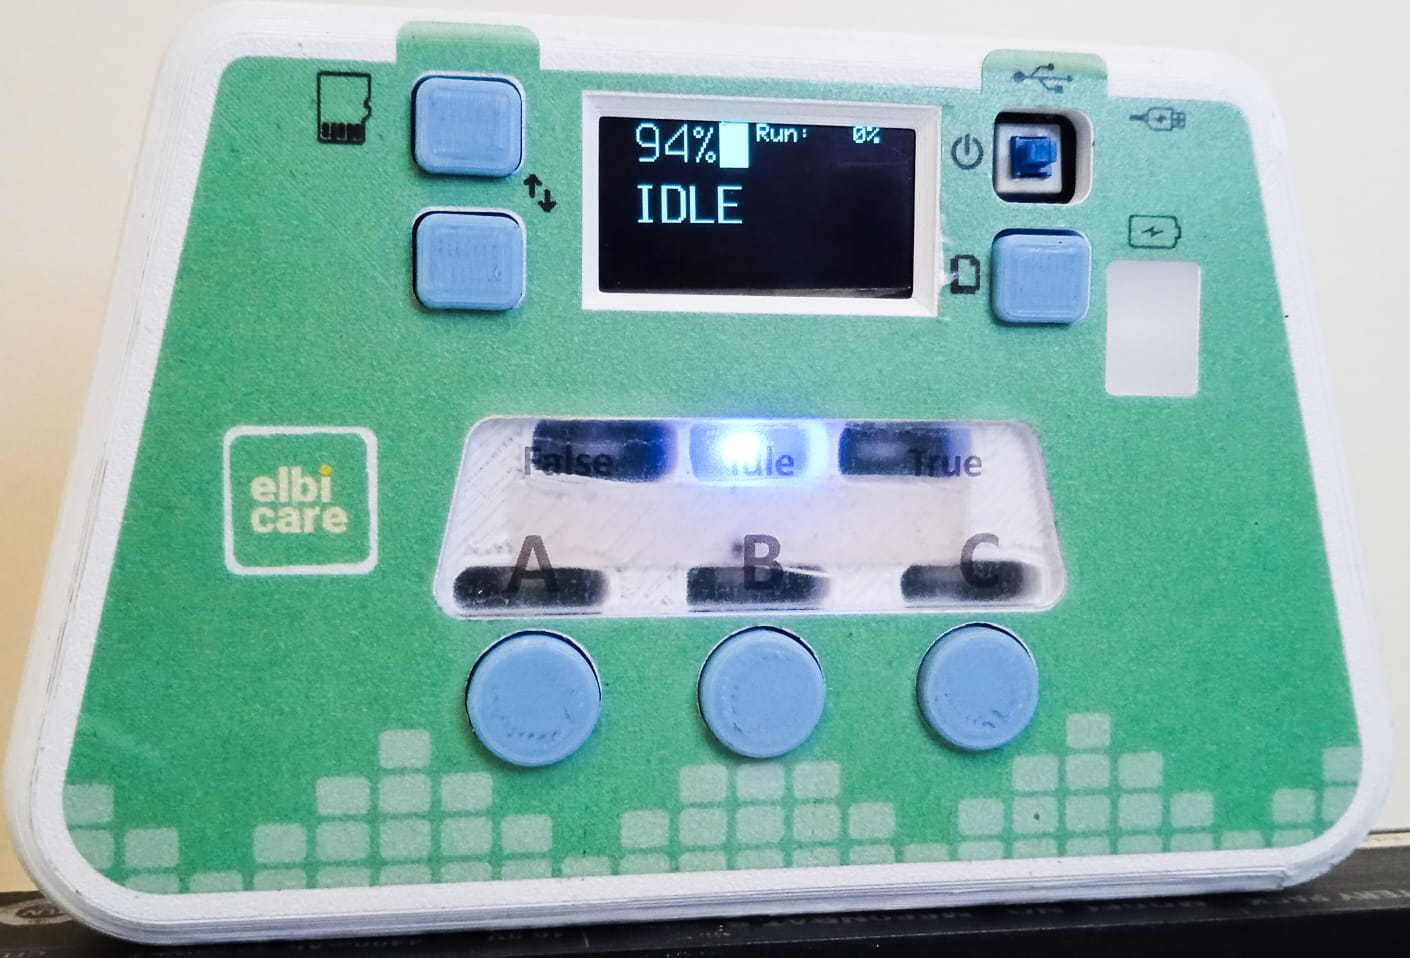
\includegraphics[width=0.7\textwidth]{images/depan-idle}
			\caption{Tampilan panel depan Elbicare Audiometers}
		\end{figure}
		
		\section{Panel Belakang}
		Panel belakang perangkat Elbicare Audiometers ditunjukkan pada Gambar berikut.
		\begin{figure}[H]
			\centering
			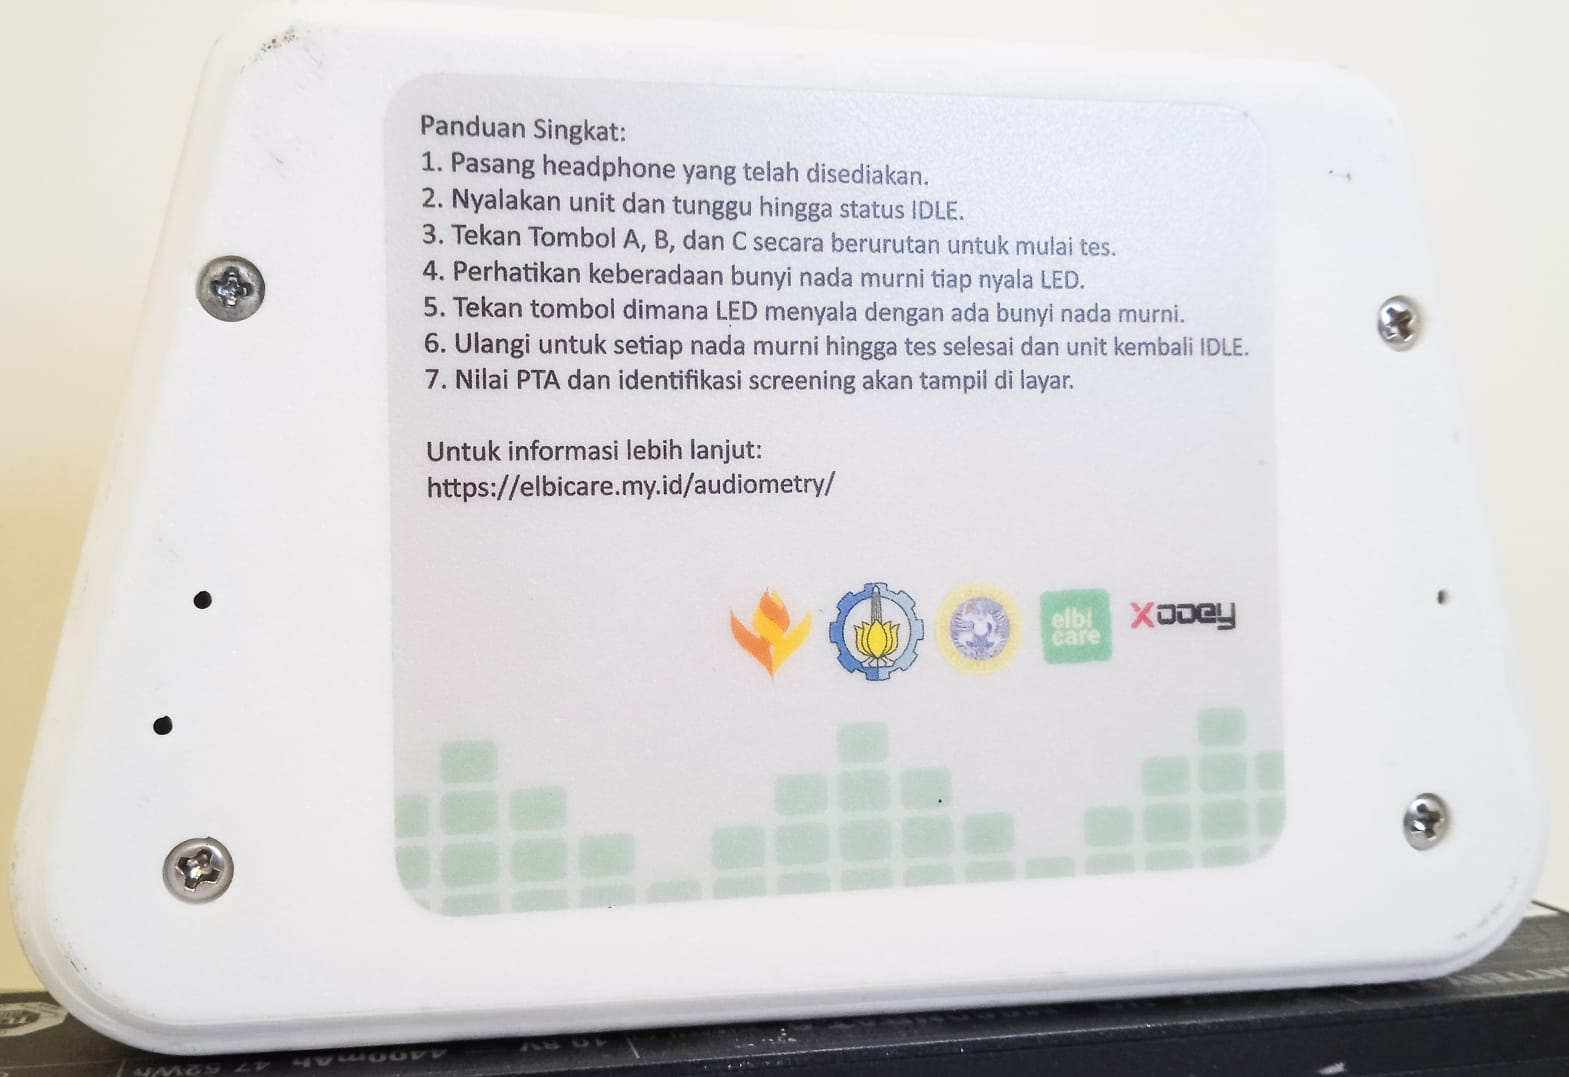
\includegraphics[width=0.7\textwidth]{images/belakang}
			\caption{Tampilan panel belakang Elbicare Audiometers}
		\end{figure}
		
		\section{Panel Atas}
		Panel atas perangkat Elbicare Audiometers ditunjukkan pada Gambar berikut.
		\begin{figure}[H]
			\centering
			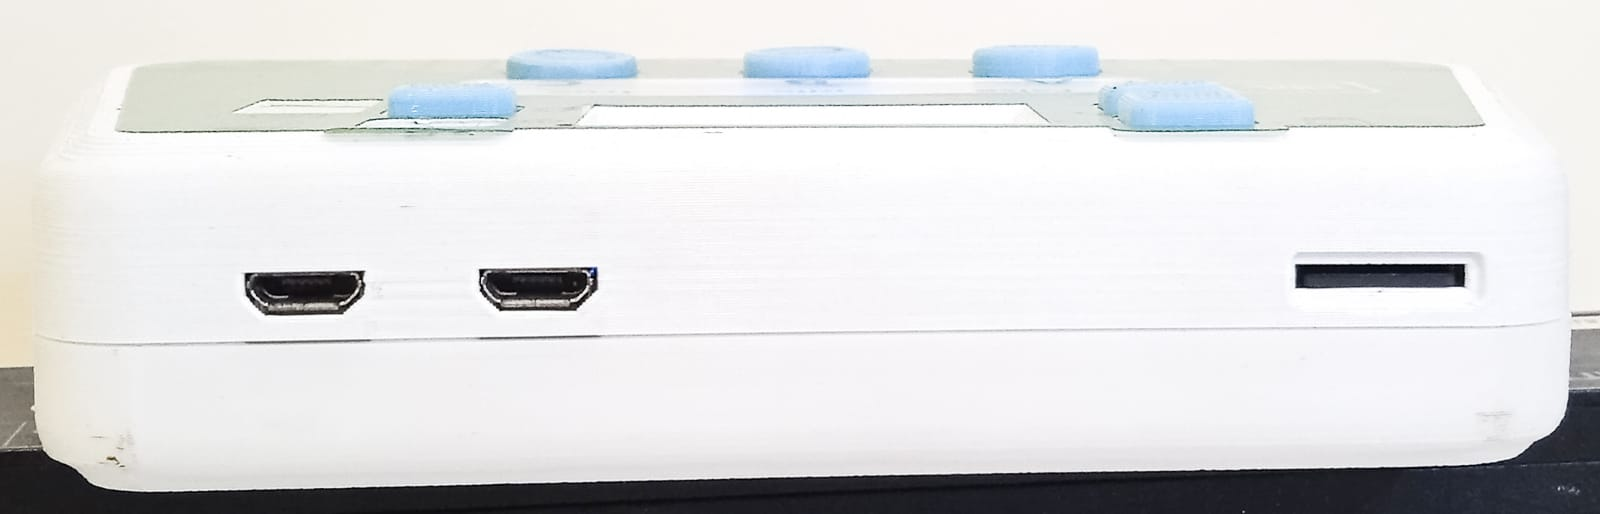
\includegraphics[width=0.7\textwidth]{images/atas}
			\caption{Tampilan panel atas Elbicare Audiometers}
		\end{figure}
		
		\section{Panel Bawah}
		Panel bawah perangkat Elbicare Audiometers ditunjukkan pada Gambar berikut.		
		\begin{figure}[H]
			\centering
			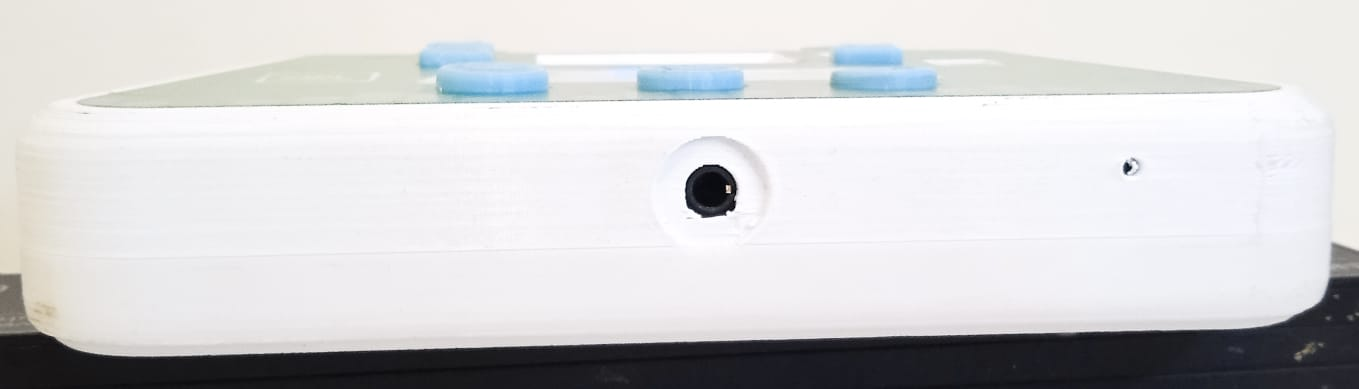
\includegraphics[width=0.7\textwidth]{images/bawah}
			\caption{Tampilan panel bawah Elbicare Audiometers}
		\end{figure}
		
		\section{Layar Tampilan}
		\subsection{Tampilan Utama}
		Tampilan utama perangkat Elbicare Audiometers ditunjukkan pada Gambar berikut.		
		\begin{figure}[H]
			\centering
			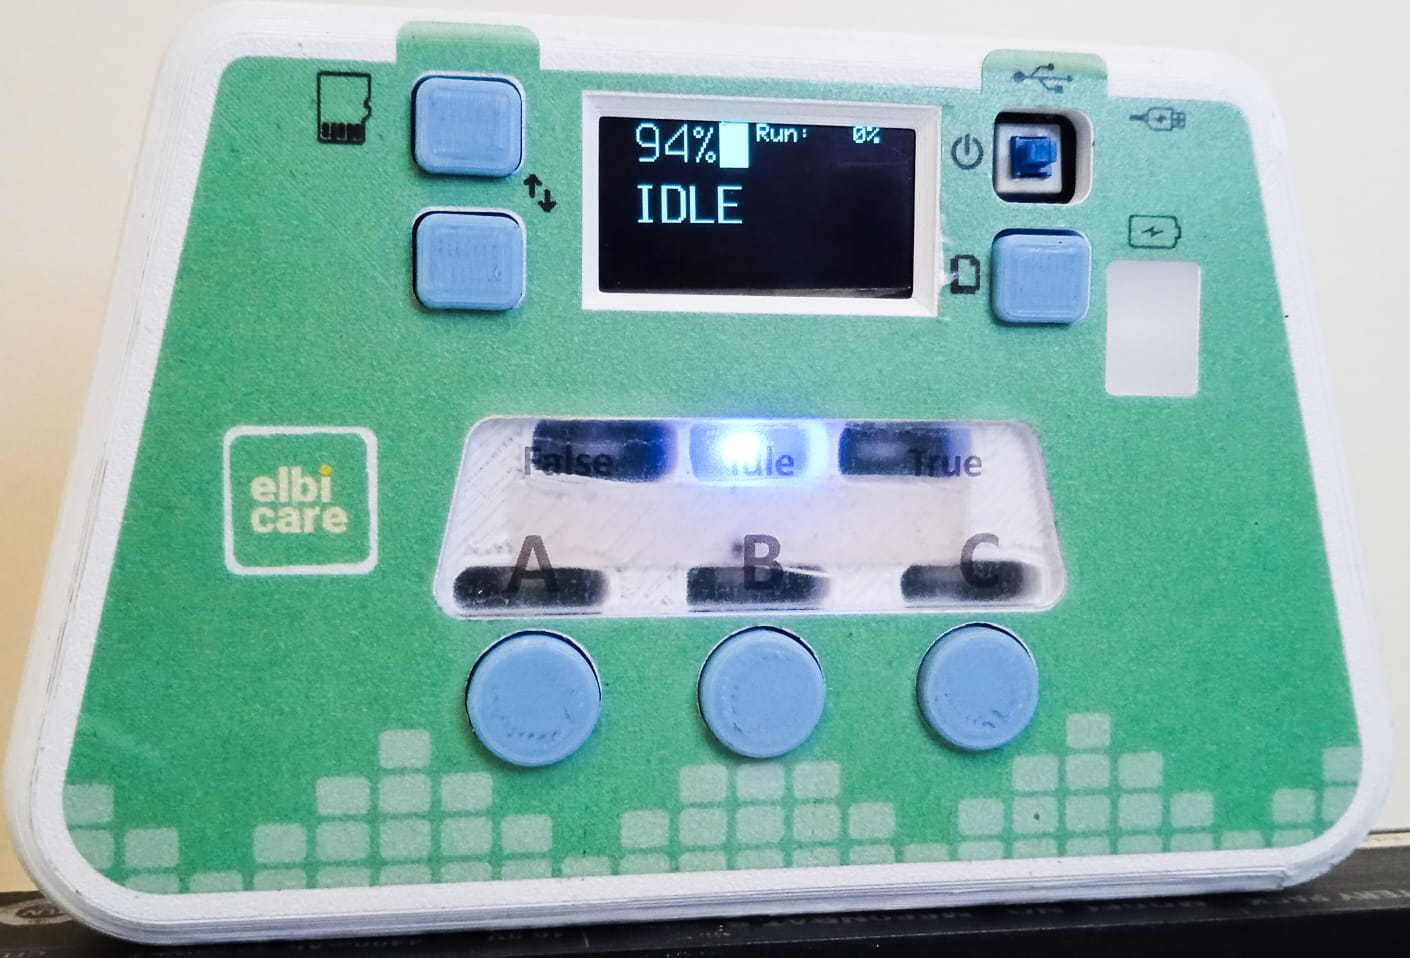
\includegraphics[width=0.7\textwidth]{images/depan-idle}
			\caption{Tampilan utama Elbicare Audiometers}
		\end{figure}	
		
		\subsection{Hasil PTA}
		Tampilan hail PTA pada perangkat Elbicare Audiometers ditunjukkan pada Gambar berikut.		
		\begin{figure}[H]
			\centering
			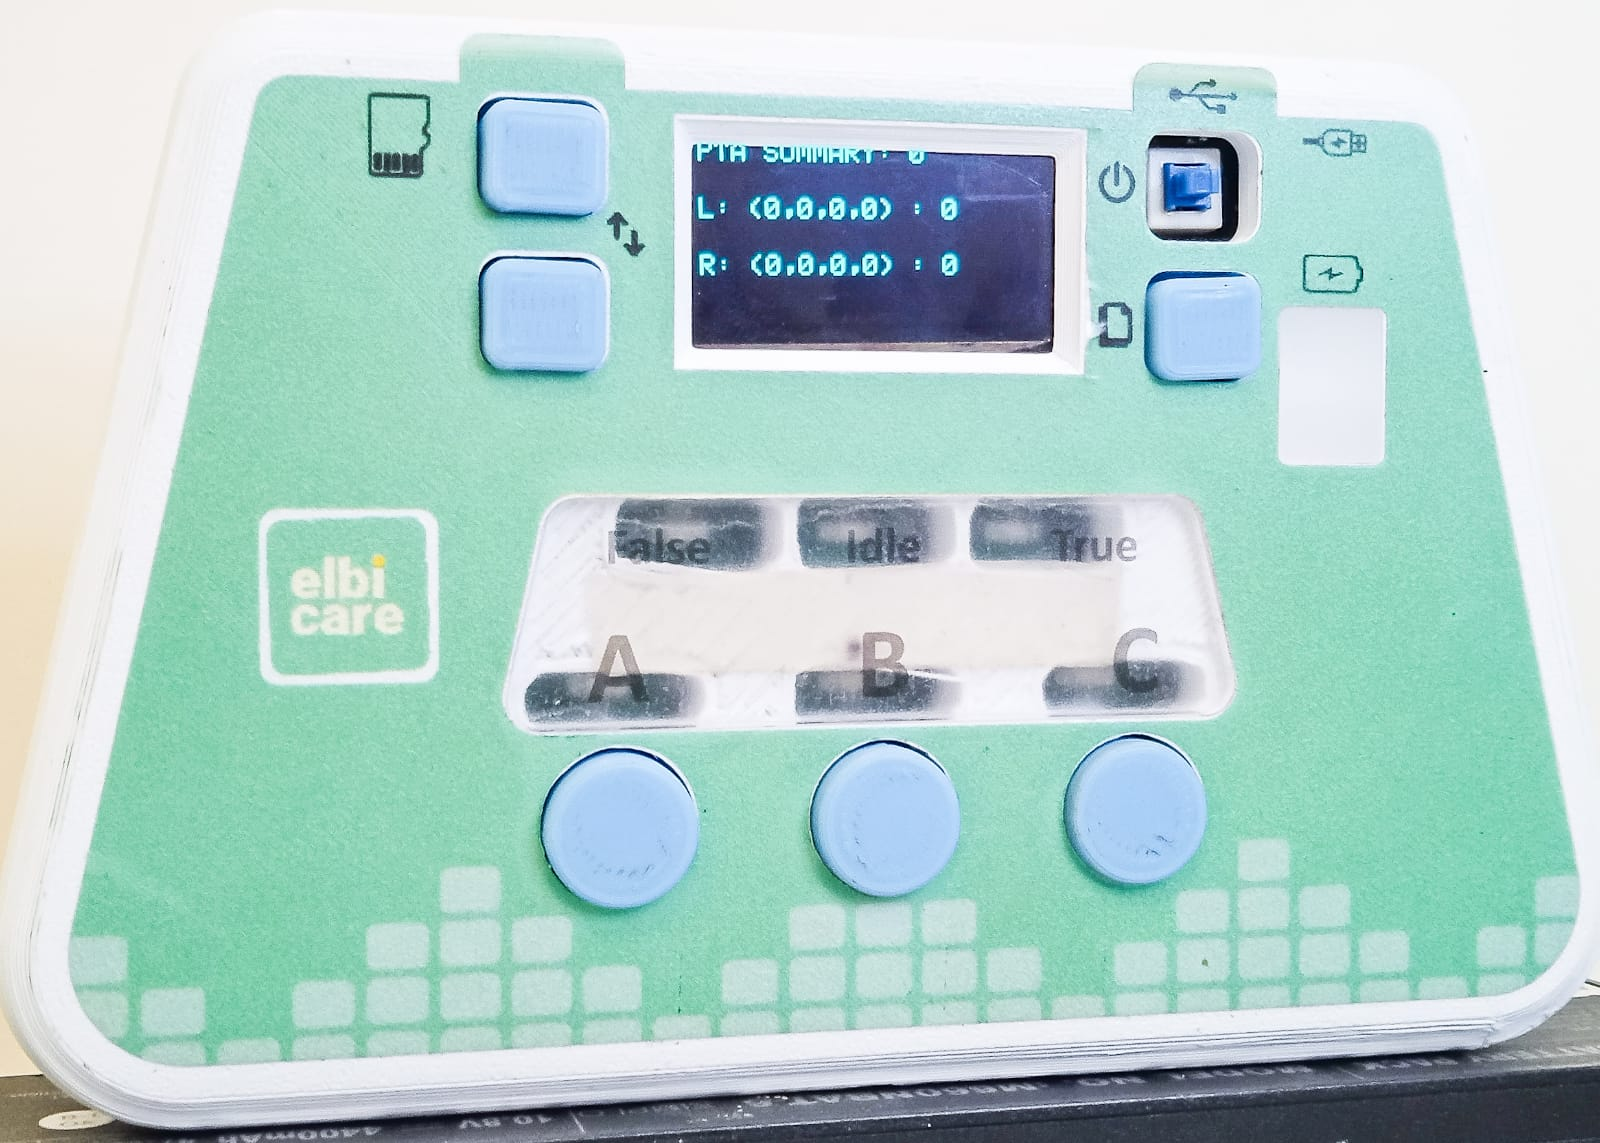
\includegraphics[width=0.7\textwidth]{images/depan-PTA}
			\caption{Tampilan hasil PTA pad Elbicare Audiometers}
		\end{figure}
		
		\section{Aksesori dan Material}
		Elbicare Audiometers menyediakan aksesori berupa
		\begin{itemize}
			\item Kabel charger
			\item Perangkat headphone JBL (wired)
			\item micro-SD
		\end{itemize}
		
		\section{Pembuangan Limbah dan Aksesori}
		Peralatan mesin dan aksesoris yang akan dibuang termasuk dalam kategori limbah B3. Peralatan mesin maupun aksesorinya harus dibuang sesuai dengan peraturan perundangan yang berlaku di Indonesia. Tata cara pembuangannya dilakukan sesuai dengan Peraturan Menteri Kesehatan Republik Indonesia.
		
	\newpage
	
%	\chapter{Troubleshooting}
%		\section{Overview}
%		\section{Troubleshooting}
%	\newpage
	
%	\chapter{Petunjuk Instalasi}
%		\section{Prosedur Instalasi Perangkat}
%		
%	\newpage
	
	\chapter{Petunjuk Pengoperasian}
		\section{Menyalakan Perangkat}
		\begin{enumerate}
			\item Melakukan instalasi perangkat sesuai petunjuk
			\item Menghubungkan headphone dengan Elbicare Audiometer
			\item Menekan tombol POWER di panel depan
		\end{enumerate}
	
		\section{Menjalankan Perangkat}
		\begin{enumerate}
			\item Memastikan kondisi perangkat dalam mode IDLE, menunjukkan slot SD Card sudah terhubung dengan perangkat
			\item Menekan tombol A, B, dan C secara berurutan 
			\item Proses audiometri secara otomatis akan berjalan, perangkat berada dalam mode RUN 
			\item Pasien menekan tombol A atau B atau C, dimana lampu led pada panel menyala diikuti dengan suara TONE
			\item Pasien memilih secara acak antara tombol A atau B atau C ketika tidak mendengar suara apapun
			\item Jawaban benar akan ditunjukkan dengan lampu led HIJAU menyala, sedangkan jawaban salah ditunjukkan dengan lampu led MERAH menyala
			\item Proses audiometri akan dimulai dengan melakukan screening pada telinga kiri, dilanjutkan dengan telinga kanan
			\item Pada setiap telinga, pasien akan diuji dengan TONE dengan frekuensi 250, 500, 1000, 2000, 4000, dan 8000 Hz, terdiri dari 11 level suara yang dikeluarkan
			\item Perangkat kembali ke mode IDLE setelah proses audiometri selesai
		\end{enumerate}
		
		\section{Mematikan Perangkat}
		\begin{enumerate}
			\item Memastikan proses audiometri tidak sedang berjalan/sudah selesai
			\item Menekan tombol POWER di panel depan
		\end{enumerate}
	
		\section{Pengumpulan Data}
		\begin{enumerate}
			\item Matikan perangkat Elbicare Audiometer
			\item Mencabut SD Card dari perangkat 
			\item Mengakses/mengambil data dalam SD Card dengan laptop/komputer menggunakan perangkat Card Reader 
		\end{enumerate}
	
	\newpage
	
	\chapter{Petunjuk Pembersihan, Sterilisasi, dan Disinfeksi}
		\section{Permukaan Perangkat}
		Penting untuk membersihkan bagian luar dan permukaan perangkat sebelum dan setelah penggunaan setiap pasien dan sesering mungkin. Pembersihan minimal dilakukan mingguan, atau kapan pun perangkat terlihat kotor.
		
		Untuk membersihkan permukaan perangkat:
		\begin{enumerate}
			\item Mencelupkan kain yang bersih dan lembut ke dalam campuran sabun dan air atau larutan pembersih lain yang ditunjukkan melalui buku panduan ini.
			\item Memeras kain untuk mengurangi kelebihan cairan.
			\item Mengusap secara perlahan bagian luar dan permukaan perangkat. Diperlukan kehati- hatian agar tidak ada cairan yang masuk ke dalam rongga permukaan.
			\item Mengeringkan permukaan perangkat dengan kain bebas serat yang kering, bersih, dan lembut.
		\end{enumerate}
		
		\begin{table}[H]
			\centering
			\caption{Larutan Pembersih yang Dapat Digunakan untuk Permukaan Perangkat}
			\label{tab:7.1}
			\begin{tabular}{|p{0.05\linewidth}  | p{0.6\linewidth}|}
				\hline
				No. & Deskripsi \\
				\hline
				\hline
				1 & Mild dishwashing detergent\\
				\hline
				2 & 70\% isopropyl alcohol (rubbing alcohol)\\
				\hline
				3 & 10\% chlorine bleach (90\% tap water)\\
				\hline
				4 & Glutaraldehyde\\
				\hline
				5 & Hospital disinfectant cleaners\\
				\hline
				6 & Hydrogen peroxide\\
				\hline
				7 & Ammonia-based household cleaners\\
				\hline
				8 & Household cleaners\\
				\hline
				9 & 15\% ammonia (85\% tap water)\\
				\hline
			\end{tabular}
		\end{table}
		
		\section{Penanganan Aksesoris}
		Pembersihan aksesoris perlu merujuk pada petunjuk yang diberikan oleh manufaktur aksesoris. 
	\newpage
	
	\chapter{Petunjuk Pemeliharaan}
	Pemeliharaan perangkat Elbicare Audiometers beserta aksesoris yang digunakan mengikuti petunjuk pada tabel berikut.
	\begin{formalblue}
		\raisebox{0.1ex}{\resizebox{!}{2.5ex}{\ding{46}}} \textbf{CATATAN}:
		Perangkat hanya boleh dibuka, direparasi, atau diservis oleh pihak yang ditunjuk secara resmi oleh \textcolor{blue}{PT. Xirka Dama Persada} 
	\end{formalblue}

	\begin{table}[H]
		\centering
		\caption{Jadwal Pemeliharaan Berkala}
		\label{tab:7.2}
		\begin{tabular}{|p{0.2\linewidth}  | p{0.2\linewidth}| p{0.4\linewidth}|}
			\hline
			Bagian & Pemeliharaan & Berkala\\
			\hline
			\hline
			Bagian panel depan dan panel belakang (casing) Elbicare Audiometer & Pembersihan area permukaan & Sesering mungkin, minimal mingguan atau setiap pergantian pengguna\\
			\hline
			Kabel charger & - & -\\
			\hline
			Micro-SD & Pemindahan data yang disimpan ke perangkat penyimpanan lain di luar perangkat Audiometers & Melalui beberapa kali pengujian, berdasarkan ukuran penyimpanan dari micro-SD yang digunakan\\
			\hline
			Headphone & Pembersihan area permukaan & Sesering mungkin, minimal mingguan atau setiap pergantian pengguna\\
			\hline
		\end{tabular}
	\end{table}

	\newpage
	
	\chapter{Lampiran}
		\section{Lampiran I: Rangkuman Spesifikasi Teknis}
		\begin{table}[H]
			\centering
			\caption{Spesifikasi teknis perangkat}
			\begin{tabular}{| l | c | r |}
				\hline
				Parts & Unit & Value \\
				\hline
				\hline
				Power voltage & $V$ & 5 \\
				\hline
				Dimensions & $mm*mm*mm$ & xx*yy*zz (without cable) \\
				\hline
				Weight & $g$ & x \\
				\hline
				Network & & IEEE 802.11b/g/n 2.4GHz \\
				\hline
				Storage & & Micro-SD Slot \\
				\hline
				Audio Port & & 3.5mm TRS \\
				\hline
				USB  Data Interface & & USB-CDC Serial \\
				\hline
				
			\end{tabular}
		\end{table}
		
	\begin{table}[H]
		\centering
		\caption{Keluaran level dari perangkat Audiometer}
		\begin{tabular}{| l | c | r |}
			\hline 
			Frequency & Tone Range(*) \\
			\hline
			\hline
			250 Hz & 17-55 dBA \\
			\hline
			500 Hz & 20-60 dBA \\
			\hline
			1000 Hz & 31-68 dBA \\
			\hline
			2000 Hz & 28-64 dBA \\
			\hline
			4000 Hz & 42-80 dBA \\
			\hline
			6000 Hz & 33-72 dBA \\
			\hline
		\end{tabular}
	\end{table}
	

%	\newpage
%		\section{Lampiran II: Diagram Sistem Elbilcare Audiometer}
		
	\newpage
	
	
	
\end{document}